\documentclass{article} % For LaTeX2e
\usepackage{nips14submit_e,times}
\usepackage{amsmath}
\usepackage{amsthm}
\usepackage{amssymb}
\usepackage{mathtools}
\usepackage{hyperref}
\usepackage{url}
\usepackage{algorithm}
\usepackage[noend]{algpseudocode}
%\documentstyle[nips14submit_09,times,art10]{article} % For LaTeX 2.09

\usepackage{graphicx}
\usepackage{caption}
\usepackage{subcaption}

\def\eQb#1\eQe{\begin{eqnarray*}#1\end{eqnarray*}}
\def\eQnb#1\eQne{\begin{eqnarray}#1\end{eqnarray}}
\providecommand{\e}[1]{\ensuremath{\times 10^{#1}}}
\providecommand{\pb}[0]{\pagebreak}
\DeclarePairedDelimiter\ceil{\lceil}{\rceil}
\DeclarePairedDelimiter\floor{\lfloor}{\rfloor}

\newcommand{\E}{\mathrm{E}}
\newcommand{\Var}{\mathrm{Var}}
\newcommand{\Cov}{\mathrm{Cov}}

\def\Qb#1\Qe{\begin{question}#1\end{question}}
\def\Sb#1\Se{\begin{solution}#1\end{solution}}

\newenvironment{claim}[1]{\par\noindent\underline{Claim:}\space#1}{}
\newtheoremstyle{quest}{\topsep}{\topsep}{}{}{\bfseries}{}{ }{\thmname{#1}\thmnote{ #3}.}
\theoremstyle{quest}
\newtheorem*{definition}{Definition}
\newtheorem*{theorem}{Theorem}
\newtheorem*{lemma}{Lemma}
\newtheorem*{question}{Question}
\newtheorem*{preposition}{Preposition}
\newtheorem*{exercise}{Exercise}
\newtheorem*{challengeproblem}{Challenge Problem}
\newtheorem*{solution}{Solution}
\newtheorem*{remark}{Remark}
\usepackage{verbatimbox}
\usepackage{listings}
\title{Probabilistic Method: \\
Problem Set IV}


\author{
Youngduck Choi \\
CIMS \\
New York University\\
\texttt{yc1104@nyu.edu} \\
}


% The \author macro works with any number of authors. There are two commands
% used to separate the names and addresses of multiple authors: \And and \AND.
%
% Using \And between authors leaves it to \LaTeX{} to determine where to break
% the lines. Using \AND forces a linebreak at that point. So, if \LaTeX{}
% puts 3 of 4 authors names on the first line, and the last on the second
% line, try using \AND instead of \And before the third author name.

\newcommand{\fix}{\marginpar{FIX}}
\newcommand{\new}{\marginpar{NEW}}

\nipsfinalcopy % Uncomment for camera-ready version

\begin{document}


\maketitle

\begin{abstract}
This work contains solutions to the problem set IV
of Probabilistic Method 2016 at Courant Institute of Mathematical Sciences.
\end{abstract}

\bigskip

\begin{question}[1]
\hfill
\begin{figure}[h!]
  \centering
    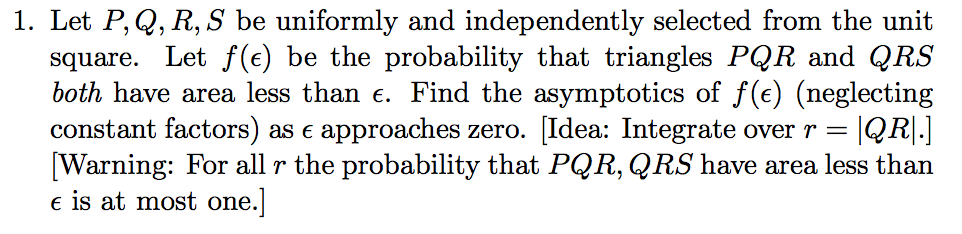
\includegraphics[width=0.7\textwidth]{PM-4-1.png}
\end{figure}
\end{question}
\newpage
\begin{solution} \hfill \\
\textbf{(1)} By elementary calculus, it follows that
\eQb
E[e^{-\lambda X_i}] &=& \int_{0}^{\infty} ae^{-(\lambda + a)t} dt \\
&=& [- \dfrac{a}{\lambda + a} e^{-(\lambda + a)t} ]_{0}^{\infty} = \dfrac{a}{\lambda + a}. 
\eQe

\smallskip

\textbf{(2)}
By (1) and mutual independence, it follows that
\eQb
E[e^{-\lambda X}] &=& E[e^{-\lambda \sum_{i=1}^{\infty} X_{i^2}}] 
= \prod_{i=1}^{\infty} E[e^{-\lambda X_{i^2}}] \\ 
&=& \prod_{i=1}^{\infty} \dfrac{i^2}{\lambda^2 +i^2}. 
\eQe


\smallskip

\textbf{(3)} Following the hint and using the Stirling's formula, we obtain
\eQb
E[e^{-K^2 X}] 
&=& \prod_{i=1}^{\infty} \dfrac{i^2}{K^2 +i^2}\\ 
&\leq& \prod_{i=1}^{K} \dfrac{i^2}{K^2 + i^2} \leq \dfrac{(k!)^2}{(k^2)^k} \\
&\sim& \dfrac{2\pi k}{e^{2k}} \\
\eQe


\smallskip

\textbf{(4)} Applying the Chernoff bound gives
\eQb
P(X \geq \epsilon) &\leq& (2\pi k) e^{\epsilon k^2 - 2k} (1 + o(1)). \\ 
\eQe
Since the quadratic is convex, we know the tightest bound is achieved at its minima, obtained
by solving for $2\epsilon k - 2 = 0$. Therefore, we have that the tightest bound is achieved with $k = 
\frac{1}{\epsilon}$, which yields
\eQb
P( X \geq \epsilon) &\leq& \dfrac{2\pi}{\epsilon} e^{-\frac{1}{\epsilon}} (1+o(1)).
\eQe

\hfill $\qed$
\end{solution}

\newpage

\begin{question}[2]
\hfill
\begin{figure}[h!]
  \centering
    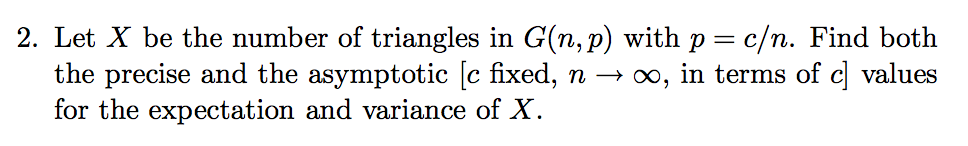
\includegraphics[width=1\textwidth]{PM-4-2.png}
\end{figure}
\end{question}
\begin{solution} 
Let $A_i$ be the subset of $\Omega$, where $I$ is the index set of all adjacent vertex pairing
in the grid. Let $B_i$ be the event where $A_i \subset C$, $X_i$ be the 
indicator random variable of $B_i$, and $X = \sum_{i \in I} X_i$, which counts the number of bonds
in a given chosen subset of $\Omega$. Counting the number of edges in the grid, it follows that
\eQb
\mu &=& \sum_{i \in I} E[X_i] = \sum_{i \in I} P(B_i) = 2n(n-1) p^2 = 2n(n-1) \dfrac{c^2}{n^2} \\ 
&\sim& 2c^2. \\
\eQe
Now, we write $i \sim j$, if $|A_i \cap A_j| = 1$. We have that
\eQb
\triangle &=& \sum_{i \sim j} P(B_i \wedge B_j). \\ 
\eQe 
Observe that $|A_i \cap A_j| = 1$ can happen in two ways: straight line or bent. The straight line
corresponds to having three consecutively chosen nodes, and the bent line means one horizontal and one
vertical bond. Observe that the bend ones can be bijected to each square excluding 1 node, and 
there are $n-2$ consecutive three nodes in each line. Therefore, we have that
\eQb
\triangle &=& \sum_{i \sim j} P(B_i \wedge B_j) = (2n(n-2) + 2(n-1)^2) p^3 \\ 
&=& (2n(n-2) + 2(n-1)^2) \dfrac{c}{n}^3 = o(1). 
\eQe
Therefore, we have shown that $\mu \to 2c^2$ as $n \to \infty$ and $\triangle = o(1)$. Hence,
by the Janson inequality(to be precise, a corollary of the inequality, which gives the
identified case as a sufficient condition for the asserted convergence), we obtain that
\eQb
P(\bigwedge_{i \in I} \overline{B_i}) \to e^{-2c^2},
\eQe
as $n \to \infty$ 
where $\bigwedge_{i \in I} \overline{B_i}$ is the event where there is no bond in both directions. 
\hfill $\qed$

\end{solution}

\newpage

\begin{question}[3]
\hfill
\begin{figure}[h!]
  \centering
    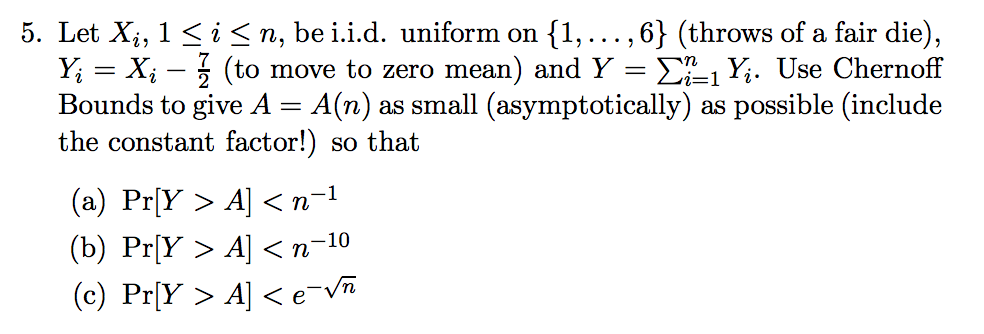
\includegraphics[width=1\textwidth]{PM-4-3.png}
\end{figure}
\end{question}
\begin{solution}
Fix $n$ and fix $\{ v, w\}$. 
Let $A_i$ be the subset of the edges of the complete graph, where $I$ is the index set of
all paths of length three, joining $v$ and $w$. 
Let $B_i$ be the event where the random graph has all the edges
of $A_i$, $X_i$ be a indicator random variable of $B_i$, and $X = \sum_{i \in I} X_i$,
which counts the number of paths of length three, joining $v$ and $w$.
The cardinality of $I$ is $2 { n -2 \choose 2 }$, which can be seen by choosing an edge,
not sharing a vertex with $\{ v , w\}$ and choosing one of two orientations that
the edge can connect to $\{ v , w\}$. Therefore, it follows that 
\eQb
\mu &=& \sum_{i \in I} E[X_i] = \sum_{i \in I} P(B_i) = 2 { n -2 \choose 2} p^3 = 2
{n - 2 \choose 2} \dfrac{c^3}{n^2}  \\
&\sim& c^3.
\eQe
Now, we write $i \sim j$, if $i \neq j$ and $A_i \cap A_j \neq \emptyset$. Observe that
as $A_i$s are the edge sets that form a path of length three, joining $u$ and $v$, we have
the following equivalence:
\eQb
i \neq j \text{ and } A_i \cap A_j = \emptyset \iff |A_i \cap A_j | = 1,
\eQe
since $|A_i \cap A_j| = 2$ implies $A_i = A_j$. We now have that 
\eQb
\triangle &=& \sum_{i \sim j} P(B_i \wedge B_j) = \sum_{|A_i \cap A_j| = 1} P(B_i \wedge B_j) \\
&=& 2{n-2 \choose 2}(1 + 2{n-4 \choose 1}) p^5  \\ 
&\sim& k n^{-\frac{1}{3}},
\eQe
where $k$ is some constant, parametrized by $c$,
as the cardinality of the ordered pair $(i,j)$ satisfying $|A_i \cap A_j| = 1$, used above,
can be seen by picking a point out side of the four vertices that that form $A_i$ path, 
and choosing one out of two possible orientations or using four vertices and choosing the opposite
orientation from itself. The above asymptotic 
immediately gives $\triangle = o(1)$.
Therefore, we have shown that $\mu \to c^3$ as $n \to \infty$ and $\triangle = o(1)$. Hence, by 
Janson's inequality (the above condition is given as sufficient condition for the convergence
below in the chapter), we obtain that 
\eQb
P(\bigwedge_{i \in I} \overline{B_i}) \to e^{-c^3},
\eQe
as $n \to \infty$ 
where $\bigwedge_{i \in I} \overline{B_i}$ is the event where there is no path of length $3$, joining
$v$ and $w$.  
\hfill $\qed$

\end{solution}

\end{document}

